\documentclass[UTF8,a4paper,12pt]{ctexart}

\usepackage{geometry}
\usepackage{amsmath}
\usepackage{amssymb}
\usepackage{graphicx}
\usepackage{booktabs}
\usepackage{float}
\usepackage{caption}
\usepackage{hyperref}
\usepackage{enumitem}
\usepackage{array}

\geometry{left=2.5cm,right=2.5cm,top=2.6cm,bottom=2.6cm}
\hypersetup{colorlinks=true,linkcolor=black,citecolor=black,urlcolor=blue}
\setlist{itemsep=0.2em,topsep=0.4em}

\title{基于机器学习的 Lorenz 混沌系统状态预测与预测边界分析}
\author{小组成员：钟兴涛、黄宇轩、郝致祺\\课程名称：人工智能导论}
\date{\today}

\begin{document}

\maketitle

\begin{abstract}
本文以 Lorenz 混沌系统为对象，研究机器学习模型对非线性动力系统短期状态转移的拟合能力及其预测边界。项目首先复现原始单变量任务，即由当前状态 $(x_t,y_t,z_t)$ 预测 $x(t+10\Delta t)$；随后将任务扩展为完整三维状态转移预测 $\mathbf{s}_t\to\mathbf{s}_{t+k}$，系统比较不同 prediction horizon、多步递归 rollout 和不同初始条件下的预测误差。进一步地，本文加入输出标准化、Residual MLP、MLP 结构与激活函数消融，以及 Echo State Network 作为动力系统时间序列模型对照。实验结果显示，Residual MLP 能显著改善中短期预测，例如 horizon=10 时 Residual MLP ReLU 64-64-64 的 state RMSE 为 0.0772，horizon=100 时为 1.4133；但当 horizon 增大到 500 时，各模型误差仍明显上升。Recursive rollout 进一步表明，一步预测模型在连续递推时会产生明显误差累积。本文结论是：机器学习可以学习 Lorenz 系统的局部短期动力学映射，模型结构改进可以扩大部分可预测时间窗，但不能因此夸大为已经解决混沌系统长期预测问题。
\end{abstract}

\noindent\textbf{关键词：} Lorenz 系统；混沌；状态转移预测；Residual MLP；Echo State Network；预测步长；递归预测；AI4SCI

\section{引言}

科学预测是人工智能与科学计算交叉领域中的重要问题。许多自然系统由确定性方程控制，但非线性耦合和初值敏感性会使其长期行为难以预测。Lorenz 系统最初来源于大气对流模型，是混沌理论中的经典案例 \cite{lorenz1963}。该系统的轨迹在相空间中形成著名的蝴蝶形吸引子，并对初始状态极其敏感。

本项目原始任务是一个较简单的短期回归问题：给定 Lorenz 系统当前状态 $(x_t,y_t,z_t)$，预测 10 个采样步长后的 $x$ 分量。该任务能够展示机器学习模型对局部非线性关系的拟合能力，但如果只报告 $R^2\approx 1$，容易将“短期局部拟合”误解为“混沌系统长期可预测”。因此，本文将研究问题从单一短期 $x$ 值预测扩展为更完整的状态转移预测与预测边界分析。

本文围绕以下问题展开：

\begin{enumerate}
    \item 机器学习模型能否从数据中学习 Lorenz 系统的完整三维状态转移映射？
    \item 当 prediction horizon 增大时，预测误差如何变化？
    \item 当 one-step 模型被递归用于 multi-step rollout 时，误差是否会累积？
    \item 在不重新训练的情况下，模型能否泛化到不同初始条件生成的新轨迹？
    \item Residual learning、输出标准化、激活函数和 ESN 是否能改善状态转移建模？
\end{enumerate}

\section{数学背景与问题定义}

\subsection{Lorenz 系统}

Lorenz 系统由以下三个耦合常微分方程组成：

\begin{equation}
\frac{dx}{dt}=\sigma(y-x),
\end{equation}

\begin{equation}
\frac{dy}{dt}=x(\rho-z)-y,
\end{equation}

\begin{equation}
\frac{dz}{dt}=xy-\beta z.
\end{equation}

本文采用经典参数设置：

\begin{equation}
\sigma=10,\quad \rho=28,\quad \beta=\frac{8}{3}.
\end{equation}

在该参数组合下，系统表现出典型混沌行为。混沌系统的关键特点是短期局部演化具有可学习规律，但长期轨迹会因初始误差和模型误差被非线性动力学放大而变得难以精确预测 \cite{strogatz2015}。

\subsection{从单变量预测到状态转移预测}

原始任务定义为：

\begin{equation}
(x_t,y_t,z_t)\rightarrow x_{t+10}.
\end{equation}

增强后的主要任务定义为完整状态转移预测。令系统状态向量为

\begin{equation}
\mathbf{s}_t=(x_t,y_t,z_t),
\end{equation}

则 prediction horizon 为 $k$ 的监督学习任务为

\begin{equation}
\mathbf{s}_t\rightarrow \mathbf{s}_{t+k}=(x_{t+k},y_{t+k},z_{t+k}).
\end{equation}

其中 $k\in\{1,5,10,20,50,100,200,500\}$。该设定比单一 $x$ 分量预测更接近动力系统状态预测任务，也能直接分析预测步长对误差的影响。

\subsection{递归 rollout}

除直接预测 $\mathbf{s}_{t+k}$ 外，本文还训练 one-step 状态转移模型：

\begin{equation}
\hat{\mathbf{s}}_{t+1}=f_\theta(\mathbf{s}_t).
\end{equation}

在 rollout 阶段，只给定初始真实状态 $\mathbf{s}_t$，之后重复使用模型输出作为下一步输入：

\begin{equation}
\hat{\mathbf{s}}_{t+i+1}=f_\theta(\hat{\mathbf{s}}_{t+i}).
\end{equation}

这一实验用于观察一步预测误差在连续递推中的累积现象。

\section{数据生成与实验设计}

\subsection{数据生成}

本文不使用外部数据集，而是通过 \texttt{scipy.integrate.solve\_ivp} 数值求解 Lorenz 方程 \cite{virtanen2020}。基础训练轨迹初始条件为 $(1,1,1)$，模拟时间范围为 $[0,50]$，采样点数为 10000，采样步长约为

\begin{equation}
\Delta t \approx 0.0050005.
\end{equation}

图 \ref{fig:lorenz} 展示了该参数设置下的三维吸引子结构。

\begin{figure}[H]
\centering
\includegraphics[width=0.78\textwidth]{figures/lorenz_attractor.png}
\caption{Lorenz 系统三维吸引子轨迹图}
\label{fig:lorenz}
\end{figure}

\subsection{模型设置}

本文比较以下模型：

\begin{enumerate}
    \item \textbf{Persistence Model}：直接将当前状态作为未来状态预测，是 naive baseline。
    \item \textbf{Linear Regression}：用线性映射近似局部状态转移，是 local linearization baseline。
    \item \textbf{Random Forest Regressor}：传统非线性机器学习强基线，参数为 \texttt{n\_estimators=300}、\texttt{max\_depth=18}、\texttt{min\_samples\_leaf=2}。
    \item \textbf{Direct MLP}：直接预测未来状态 $\mathbf{s}_{t+k}$，用于和原始 MLP 设置对照。
    \item \textbf{Residual MLP}：预测状态变化量 $\Delta\mathbf{s}=\mathbf{s}_{t+k}-\mathbf{s}_t$，再还原 $\hat{\mathbf{s}}_{t+k}=\mathbf{s}_t+\widehat{\Delta\mathbf{s}}$。该设计更贴近数值积分中的“当前状态加增量”思想。
    \item \textbf{Echo State Network}：使用固定随机 reservoir 和线性 readout 的 reservoir computing 模型，作为动力系统时间序列模型对照。
\end{enumerate}

模型使用 scikit-learn 实现 \cite{pedregosa2011}；Echo State Network 使用轻量 NumPy 实现。对输入特征使用 StandardScaler 标准化，且只在训练集上 fit，再应用到测试集。对 MLP 的输出目标 $Y=(x,y,z)$ 或残差目标 $\Delta Y$ 也使用 StandardScaler，并在评价前 inverse transform 回原始物理尺度，以避免不同状态分量的数值尺度影响训练。

\subsection{评价指标}

对单变量原始任务，继续使用 RMSE、MAE 和 $R^2$。对完整三维状态预测，本文定义 state RMSE：

\begin{equation}
RMSE_{state}=\sqrt{\frac{1}{n}\sum_{i=1}^{n}\|\mathbf{s}_i-\hat{\mathbf{s}}_i\|_2^2}.
\end{equation}

同时计算 $x,y,z$ 各分量的 RMSE、MAE、$R^2$，并报告三个分量 $R^2$ 的平均值 $R^2_{mean}$。

\section{实验结果}

\subsection{原始单变量短期预测结果}

表 \ref{tab:original_metrics} 给出了原始 $x(t+10\Delta t)$ 预测任务结果。非线性模型在该任务上取得很高精度，说明 Lorenz 系统短期局部演化映射可以被机器学习模型拟合。

\begin{table}[H]
\centering
\caption{原始单变量短期预测结果}
\label{tab:original_metrics}
\begin{tabular}{lccc}
\toprule
模型 & RMSE & MAE & $R^2$ \\
\midrule
Persistence Model & 2.1653 & 1.7657 & 0.9208 \\
线性回归 & 0.5679 & 0.4556 & 0.9946 \\
随机森林 & 0.0887 & 0.0504 & 0.9999 \\
MLP & 0.0779 & 0.0574 & 0.9999 \\
\bottomrule
\end{tabular}
\end{table}

但是，该结果只说明固定短 horizon 和单一 $x$ 分量预测较容易，并不能代表长期混沌预测已经被解决。

\subsection{Prediction horizon sensitivity}

表 \ref{tab:horizon_metrics} 展示了若干关键 horizon 下的三维状态预测结果。可以看到，horizon=10 时 Random Forest 和 MLP 均能保持较低 state RMSE；当 horizon 增大到 100 和 500 后，误差显著增加，$R^2_{mean}$ 也明显下降。

\begin{table}[H]
\centering
\caption{不同 prediction horizon 下的三维状态预测结果}
\label{tab:horizon_metrics}
\begin{tabular}{rlcc}
\toprule
Horizon & 模型 & State RMSE & $R^2_{mean}$ \\
\midrule
10 & Random Forest & 0.2987 & 0.9996 \\
10 & MLP & 0.4572 & 0.9991 \\
100 & Random Forest & 4.3280 & 0.9164 \\
100 & MLP & 2.2369 & 0.9781 \\
500 & Random Forest & 12.7868 & 0.2607 \\
500 & MLP & 13.6858 & 0.1591 \\
\bottomrule
\end{tabular}
\end{table}

图 \ref{fig:horizon_rmse} 更直观地展示了 horizon 与 state RMSE 的关系。随着 prediction horizon 增大，Persistence 和 Linear Regression 快速失效；非线性模型在中短期内更稳健，但在较长 horizon 下也出现明显退化。

\begin{figure}[H]
\centering
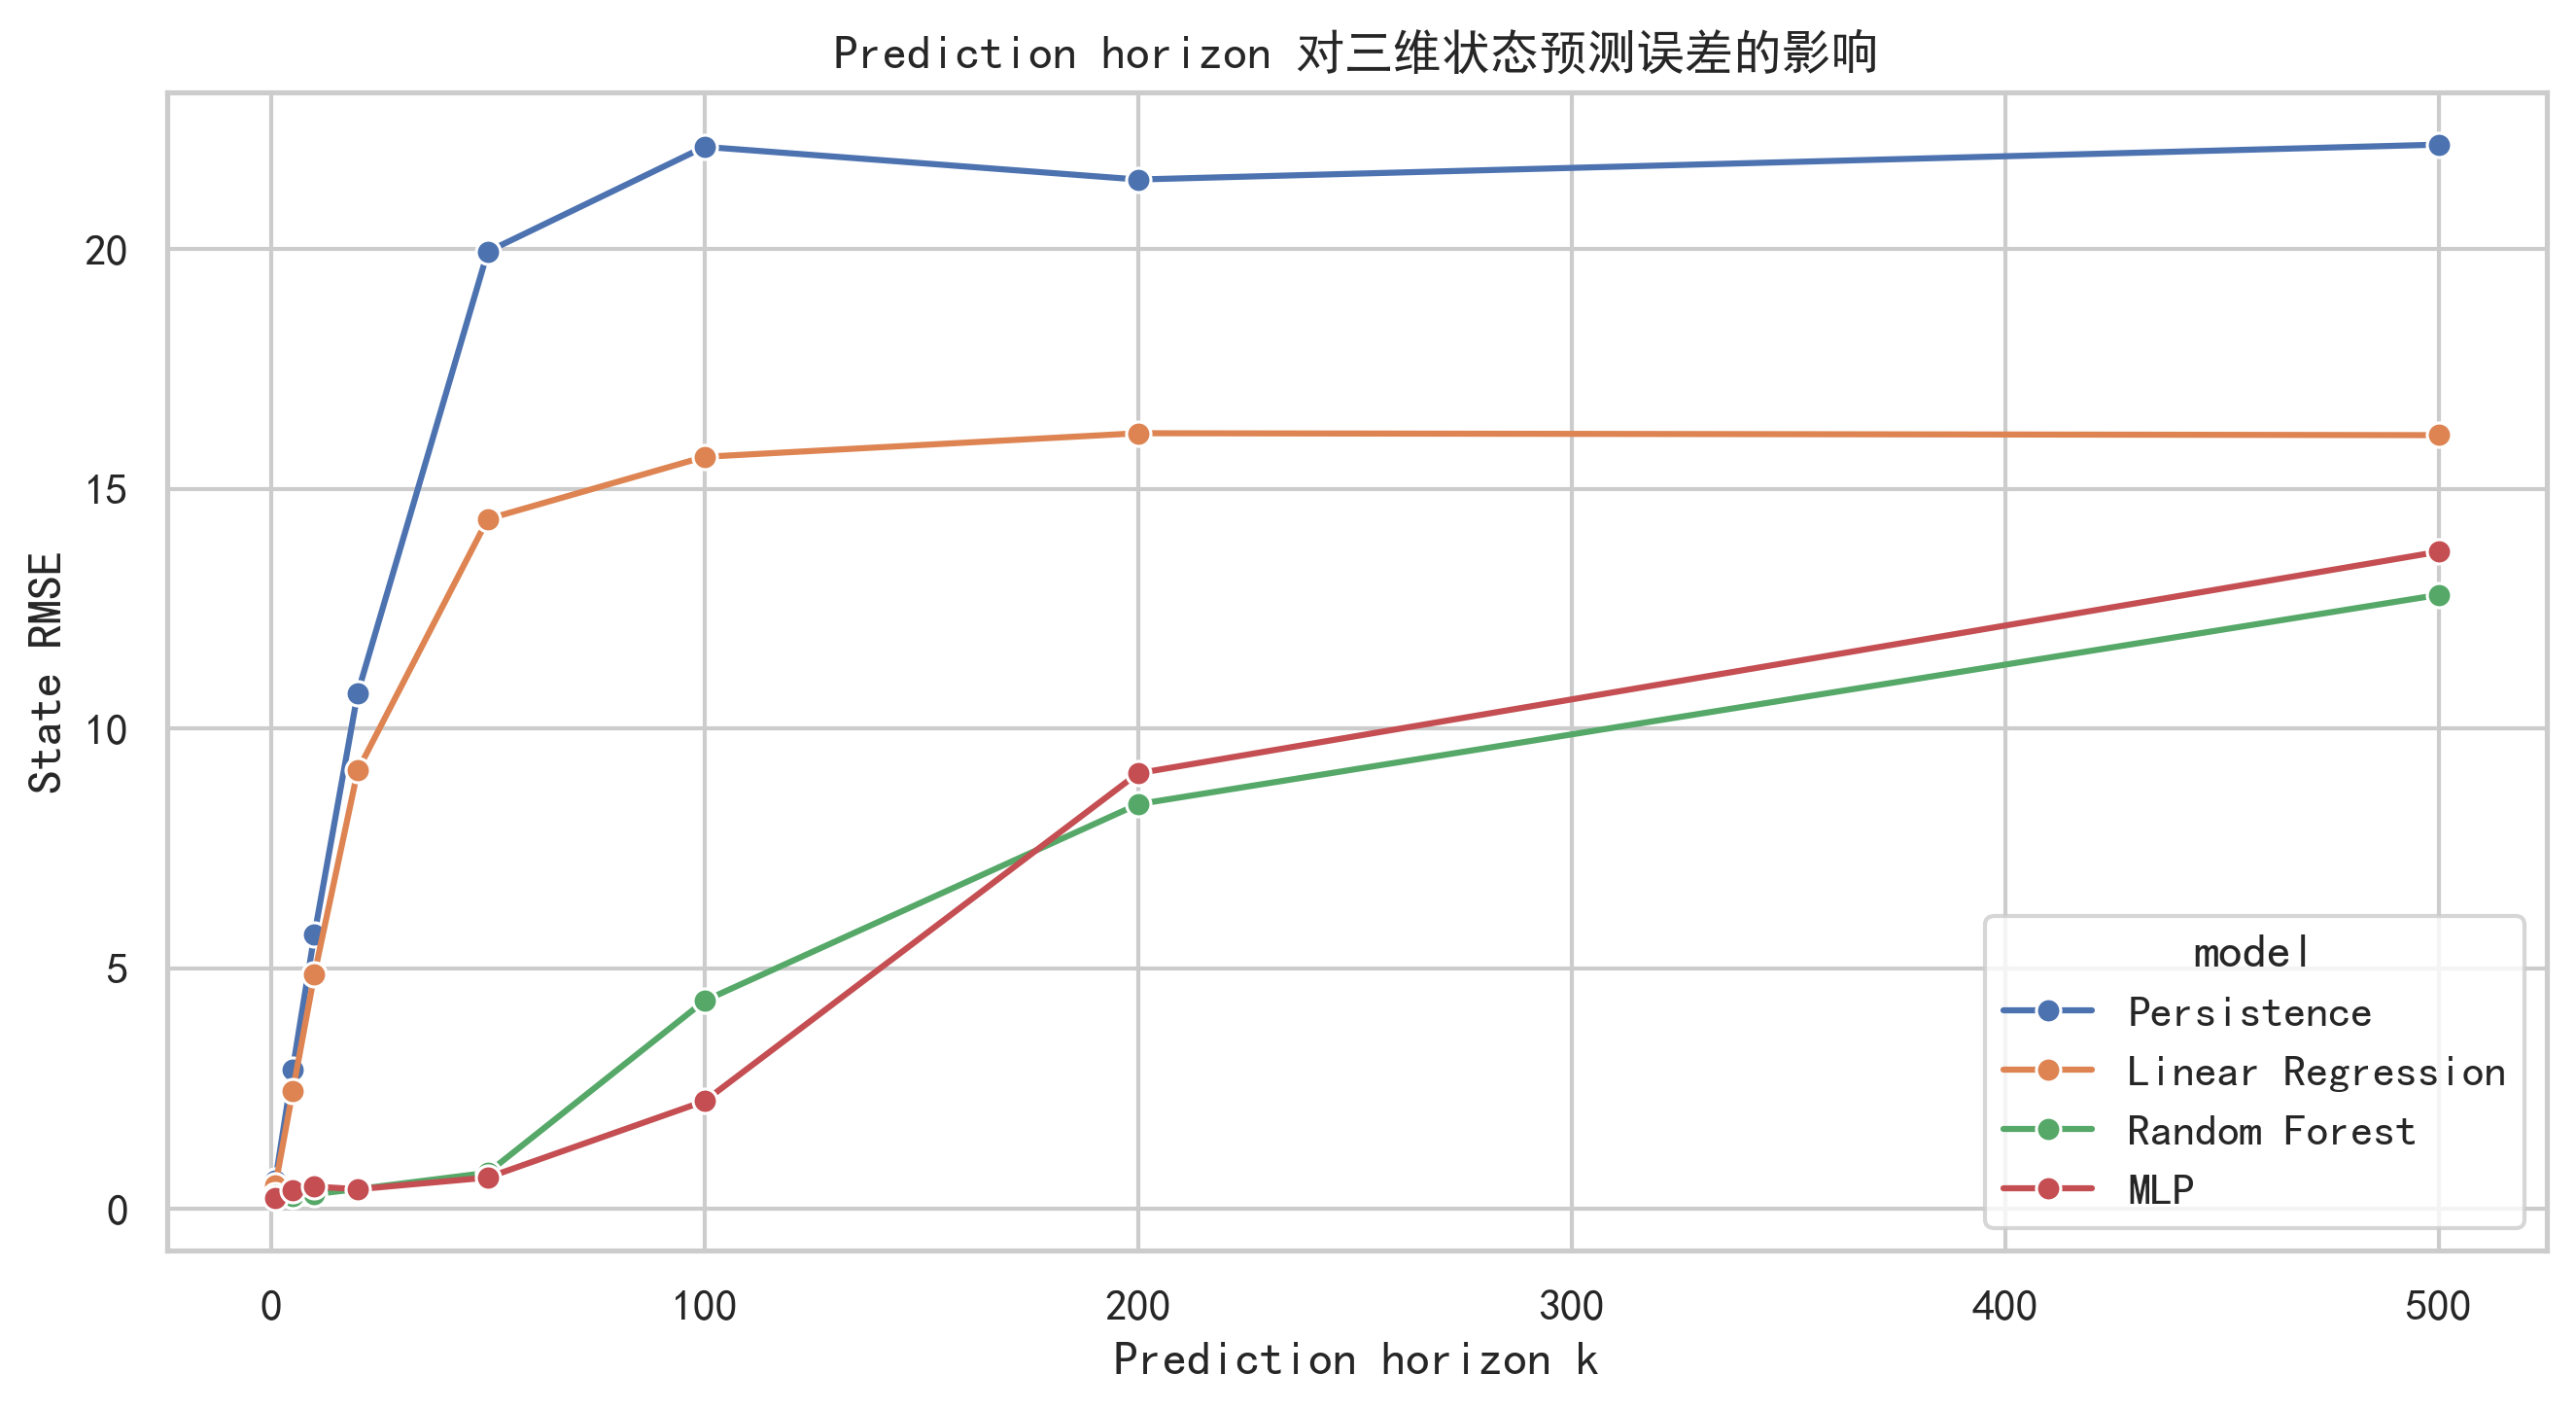
\includegraphics[width=0.86\textwidth]{figures/horizon_vs_rmse.png}
\caption{Prediction horizon 对三维状态预测误差的影响}
\label{fig:horizon_rmse}
\end{figure}

\subsection{Recursive multi-step rollout}

直接预测 $\mathbf{s}_{t+k}$ 仍然使用真实当前状态作为输入，而实际长期预测更接近 recursive rollout：模型必须不断使用自己的预测结果继续向前推演。图 \ref{fig:rollout_error} 显示了 500 步 rollout 中累计 state RMSE 的变化。500 步结束时，Linear Regression、Random Forest、MLP 的累计 state RMSE 分别约为 20.2040、14.3255、18.0711。

\begin{figure}[H]
\centering
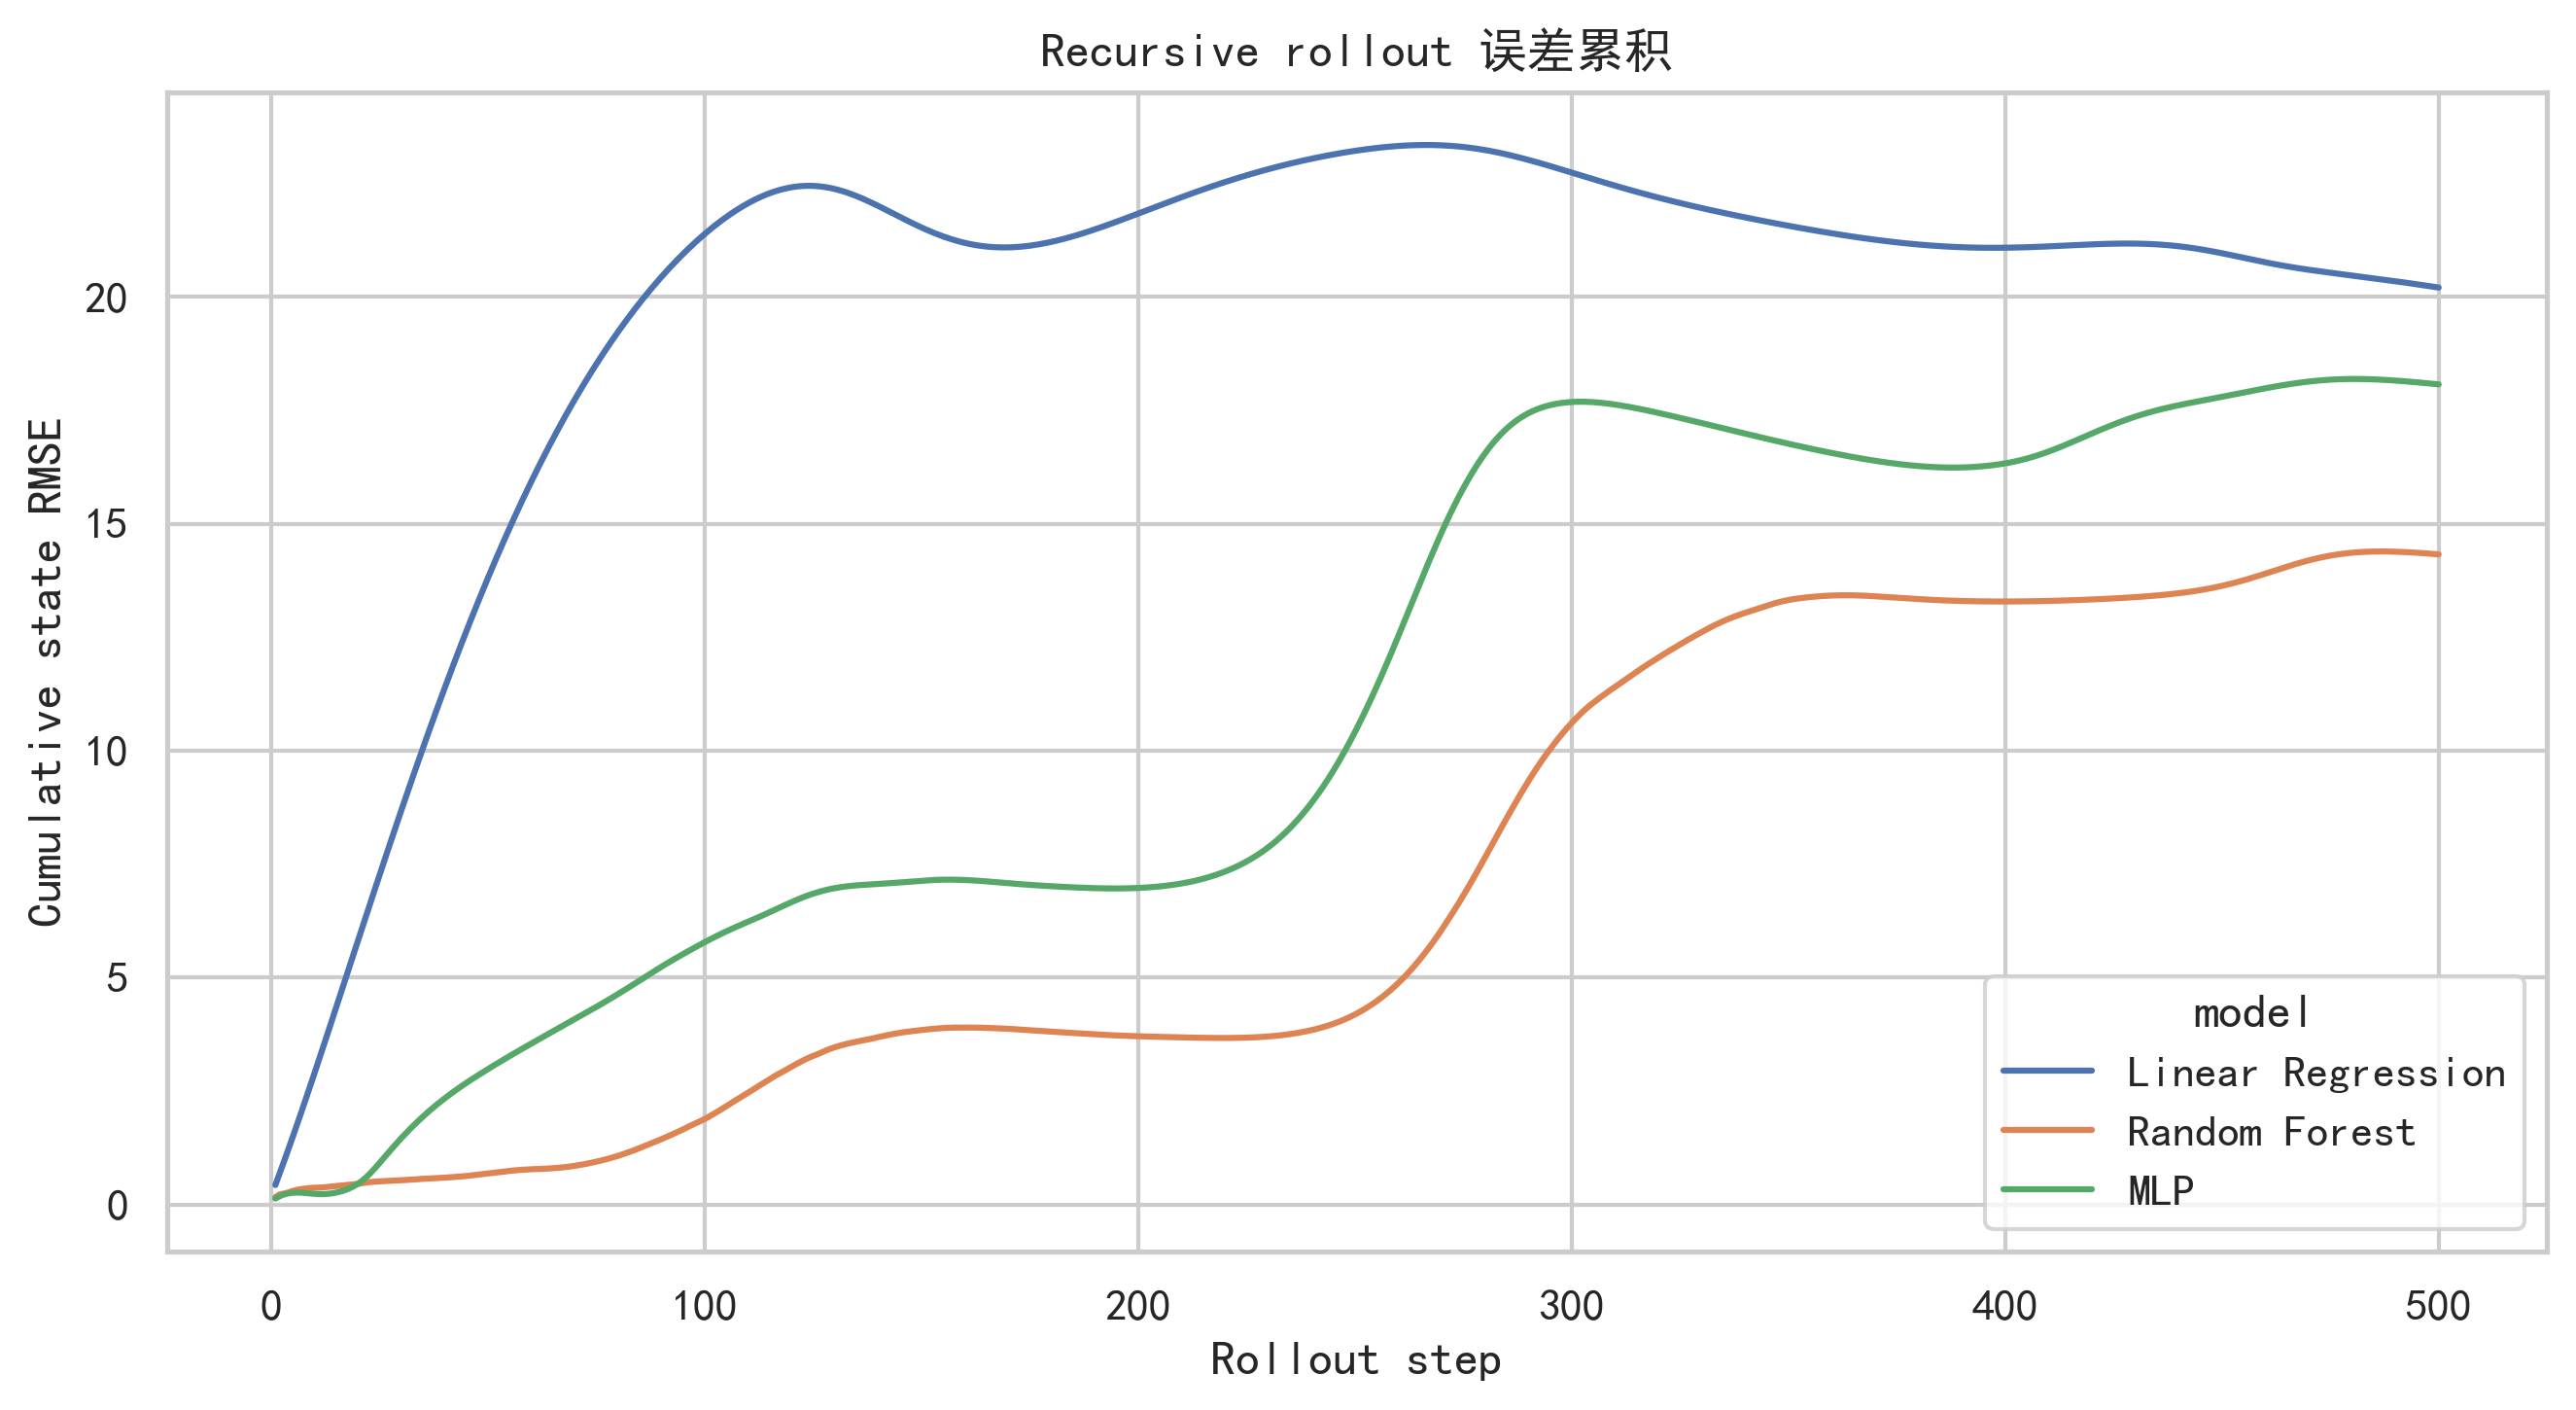
\includegraphics[width=0.86\textwidth]{figures/rollout_error.png}
\caption{Recursive rollout 中的误差累积曲线}
\label{fig:rollout_error}
\end{figure}

图 \ref{fig:rollout_x} 展示了 rollout 中 $x(t)$ 的真实值与预测值对比。即使 one-step 模型在短期预测上表现较好，连续递推后仍会逐渐偏离真实轨迹。

\begin{figure}[H]
\centering
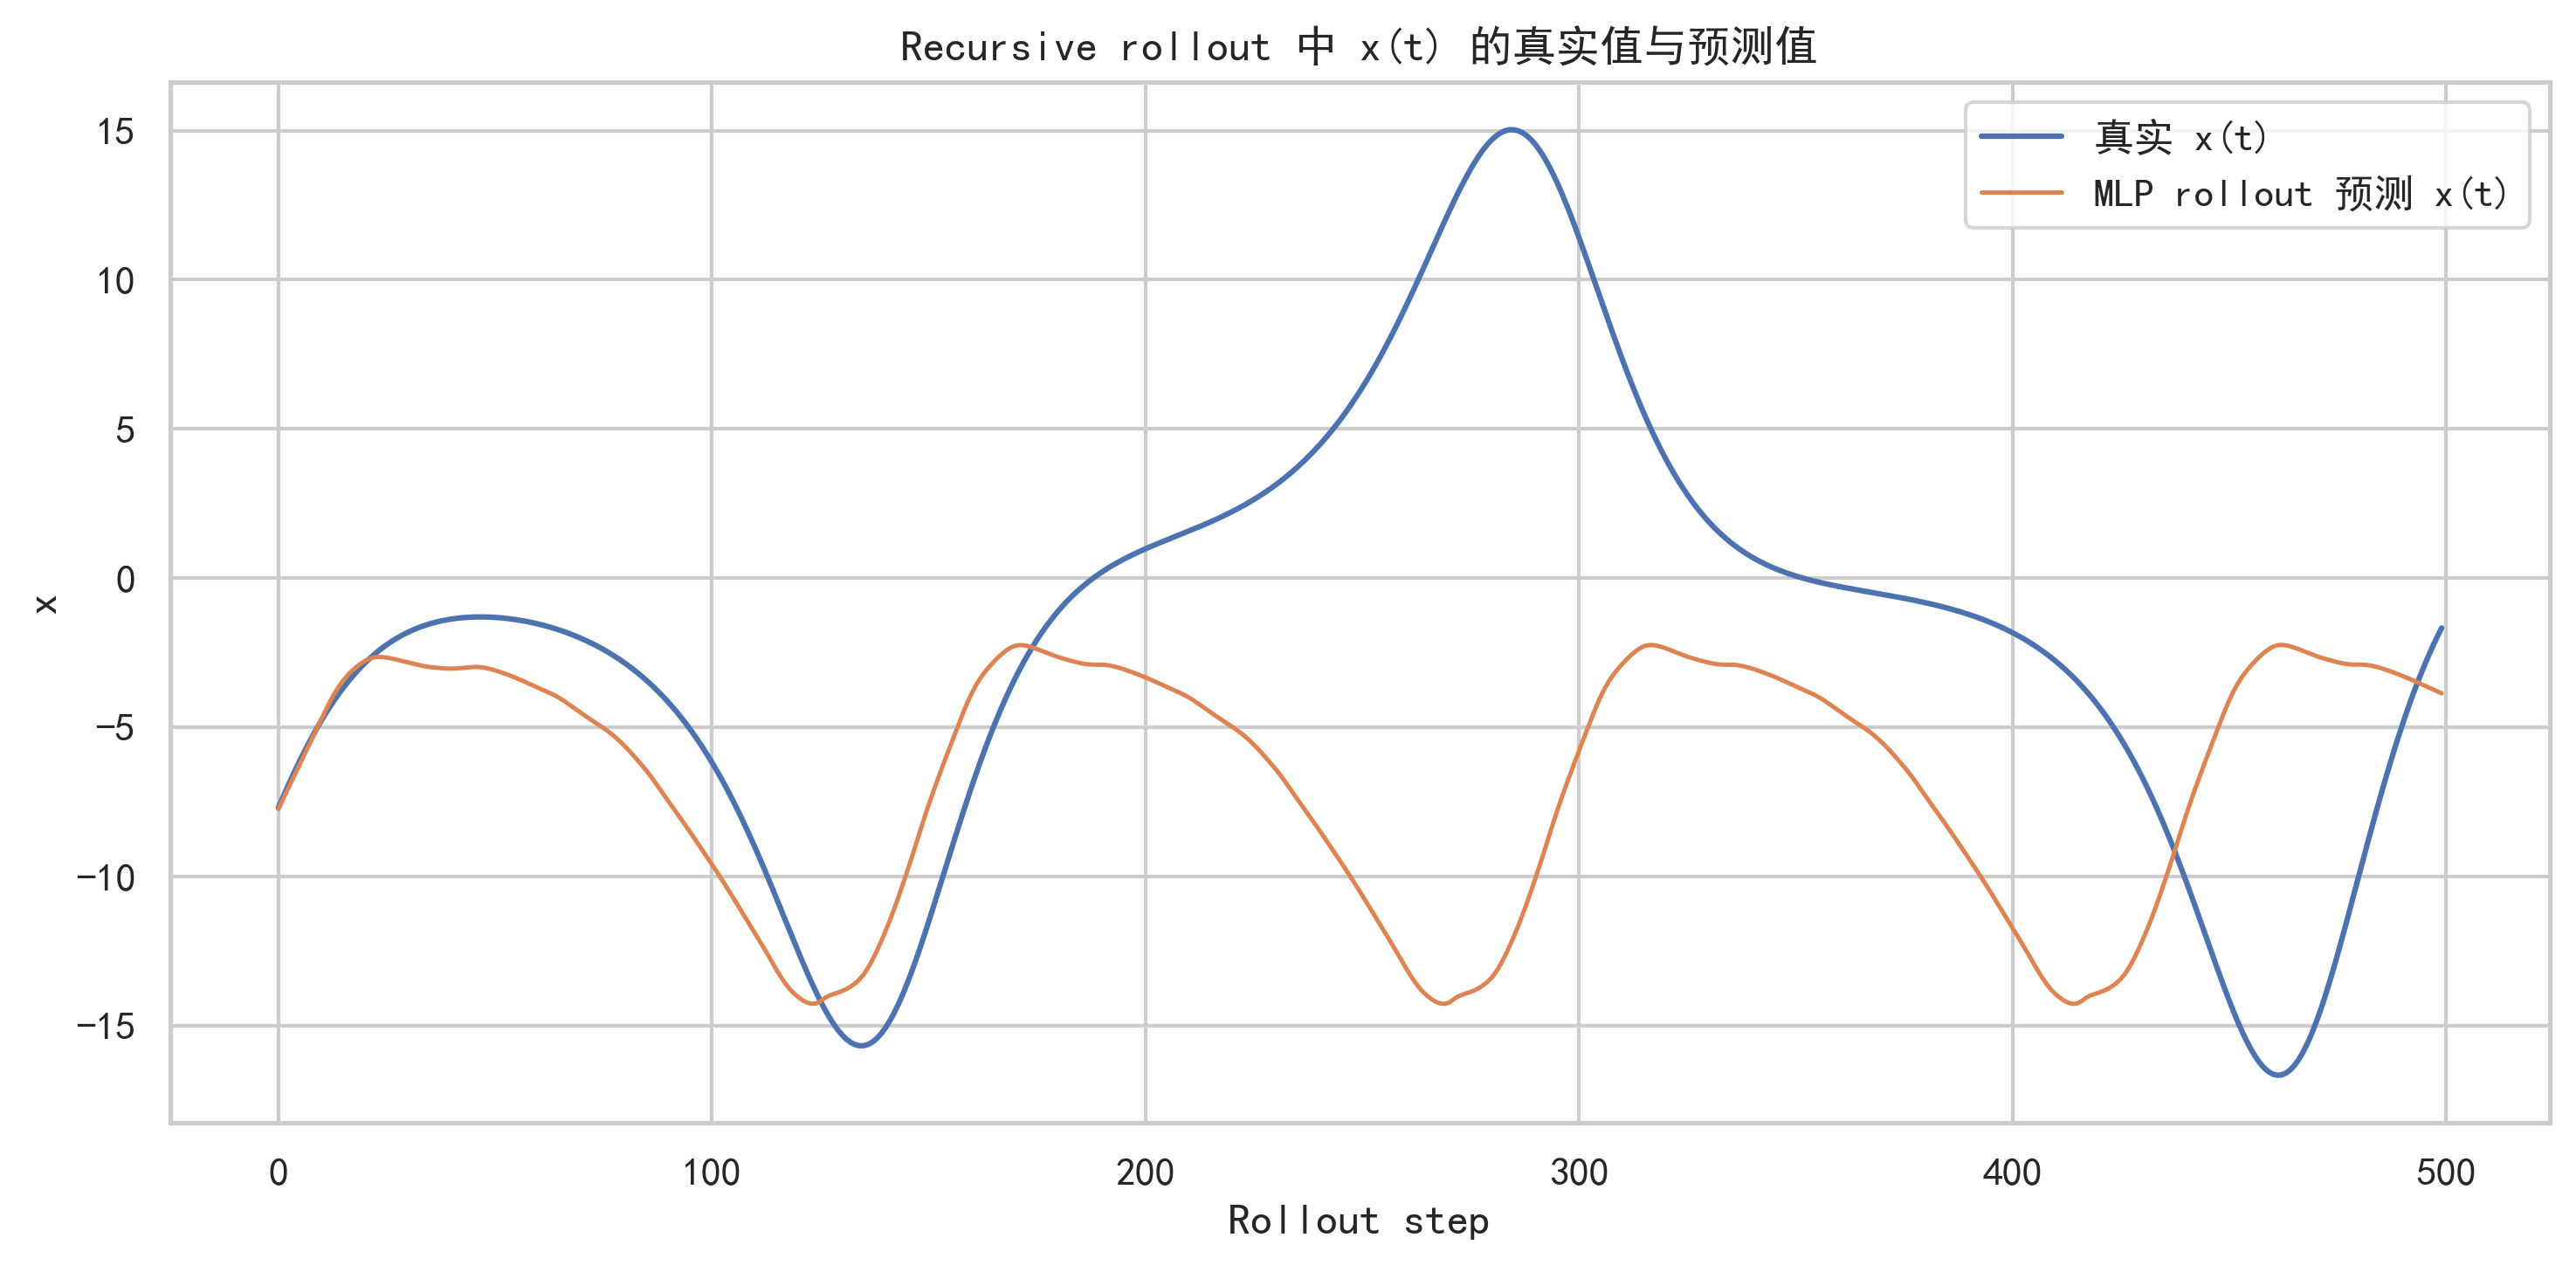
\includegraphics[width=0.86\textwidth]{figures/rollout_x_comparison.png}
\caption{Recursive rollout 中 $x(t)$ 的真实值与预测值对比}
\label{fig:rollout_x}
\end{figure}

图 \ref{fig:rollout_attractor} 从三维相空间角度比较真实轨迹与 rollout 预测轨迹。该图说明点预测误差的累积会进一步表现为相空间轨迹的偏移。

\begin{figure}[H]
\centering
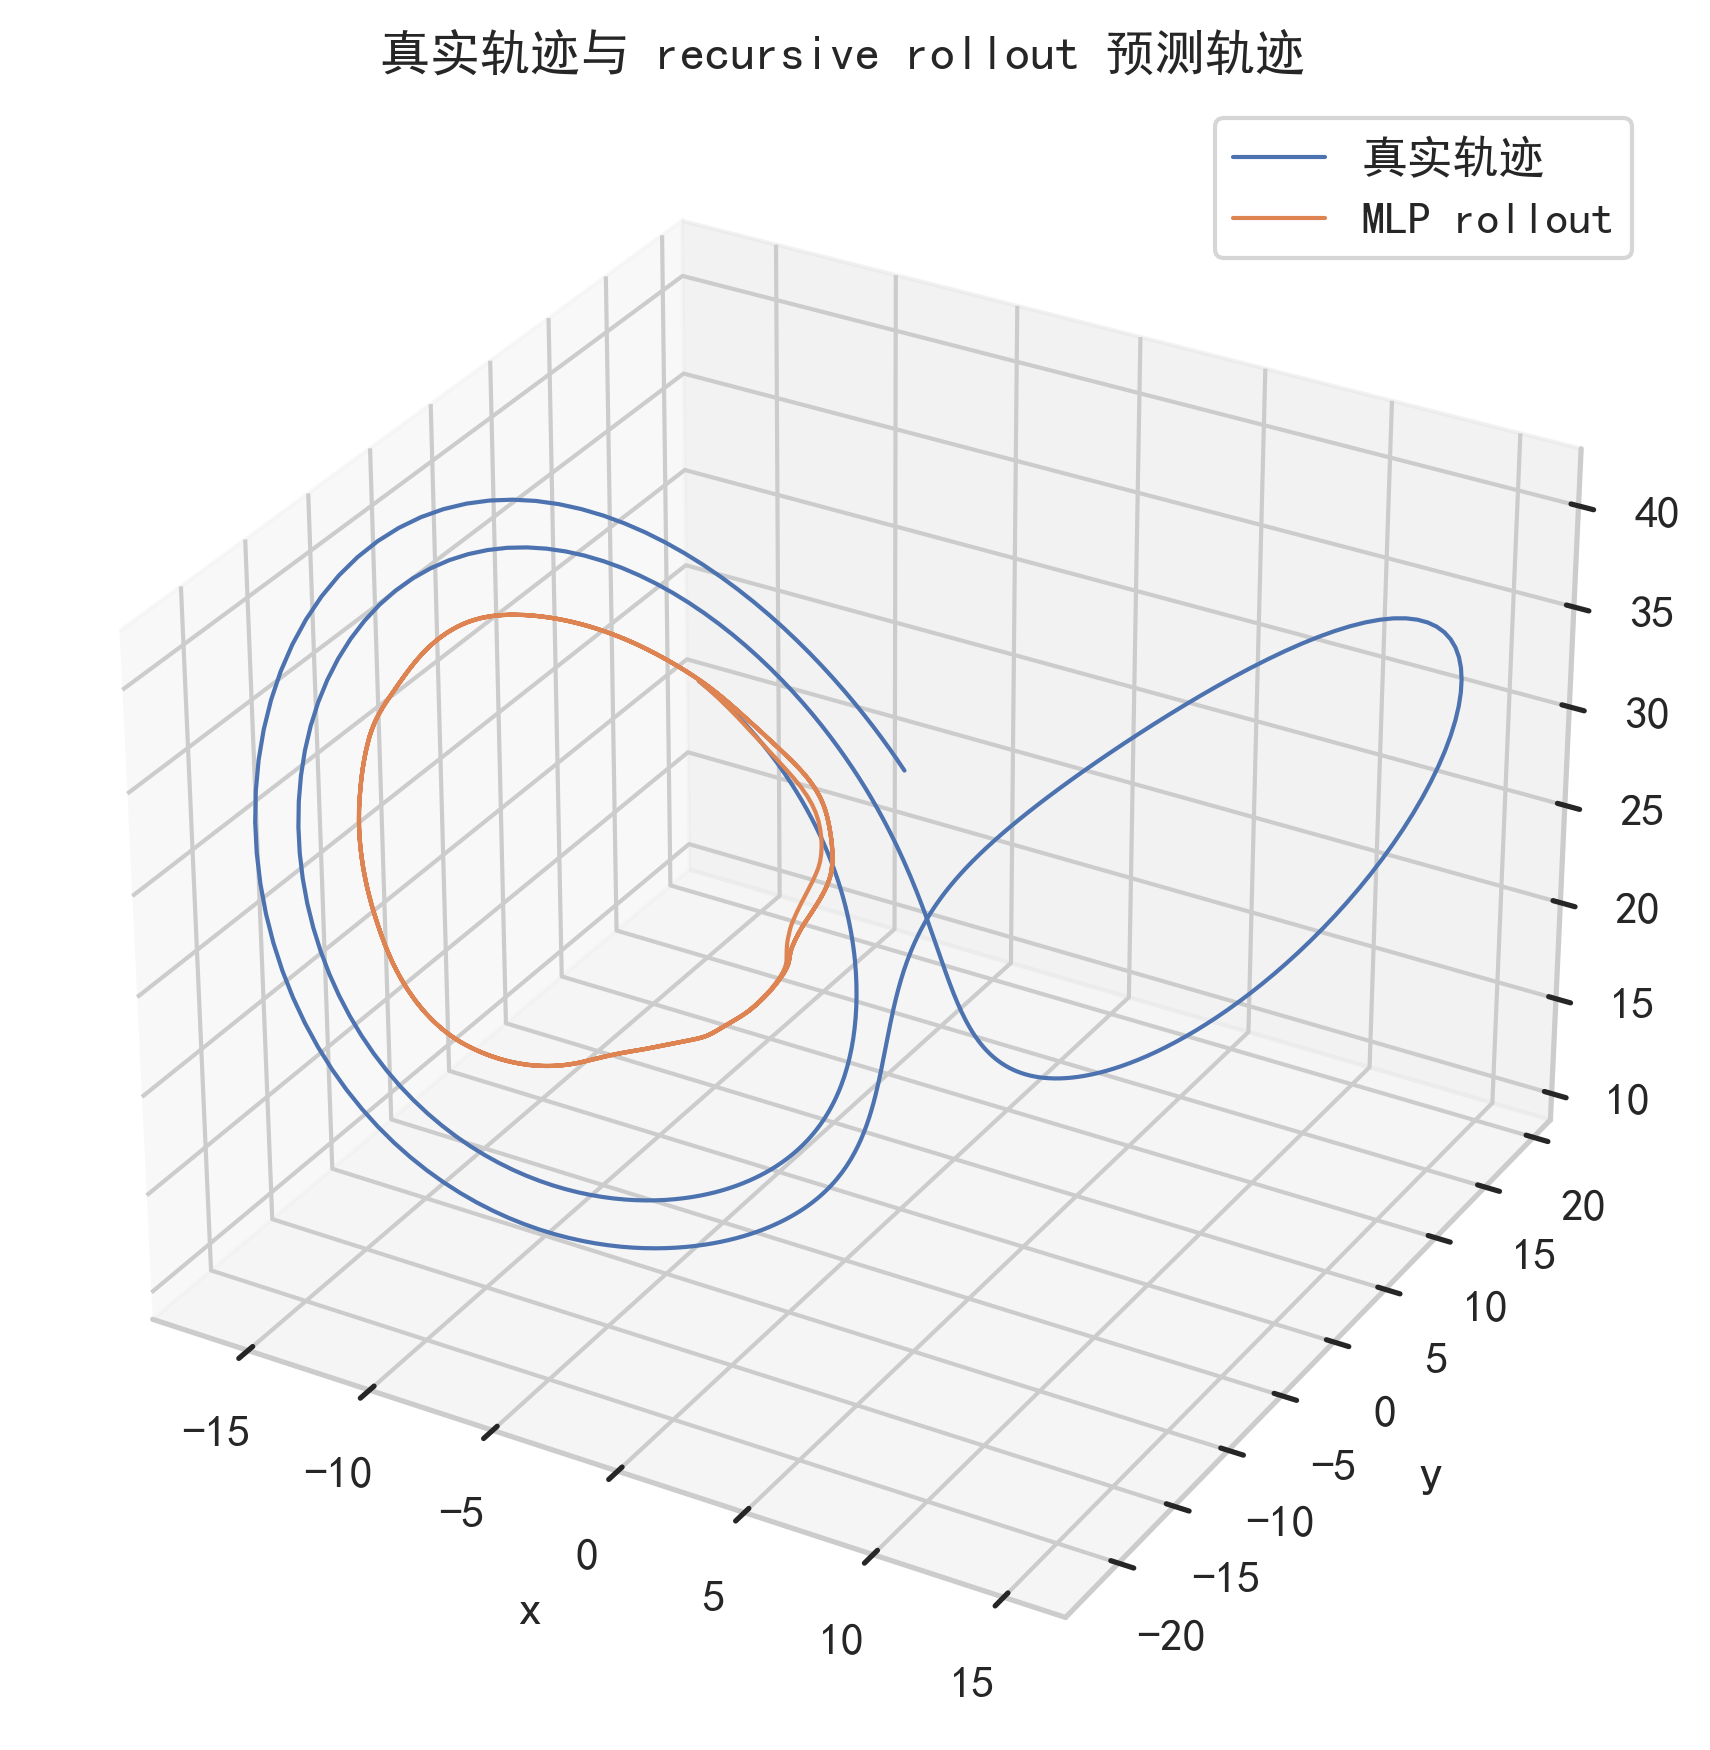
\includegraphics[width=0.78\textwidth]{figures/rollout_attractor.png}
\caption{真实轨迹与 recursive rollout 预测轨迹的三维对比}
\label{fig:rollout_attractor}
\end{figure}

\subsection{Initial-condition generalization}

为了测试模型是否只是拟合同一条轨迹，本文保持模型训练数据主要来自初始条件 $(1,1,1)$，然后直接测试其他初始条件生成的轨迹，不进行重新训练。测试初始条件包括 $(1.01,1,1)$、$(1.1,1,1)$、$(-5,5,20)$ 和 $(10,10,10)$。

图 \ref{fig:ic_rmse} 展示了不同初始条件下的 state RMSE。结果表明，非线性模型在新初值轨迹上仍明显优于 Persistence 和 Linear Regression，但误差水平会随初始条件和轨迹分布变化而波动。这说明模型具有一定局部泛化能力，但其泛化仍受到训练轨迹覆盖范围限制。

\begin{figure}[H]
\centering
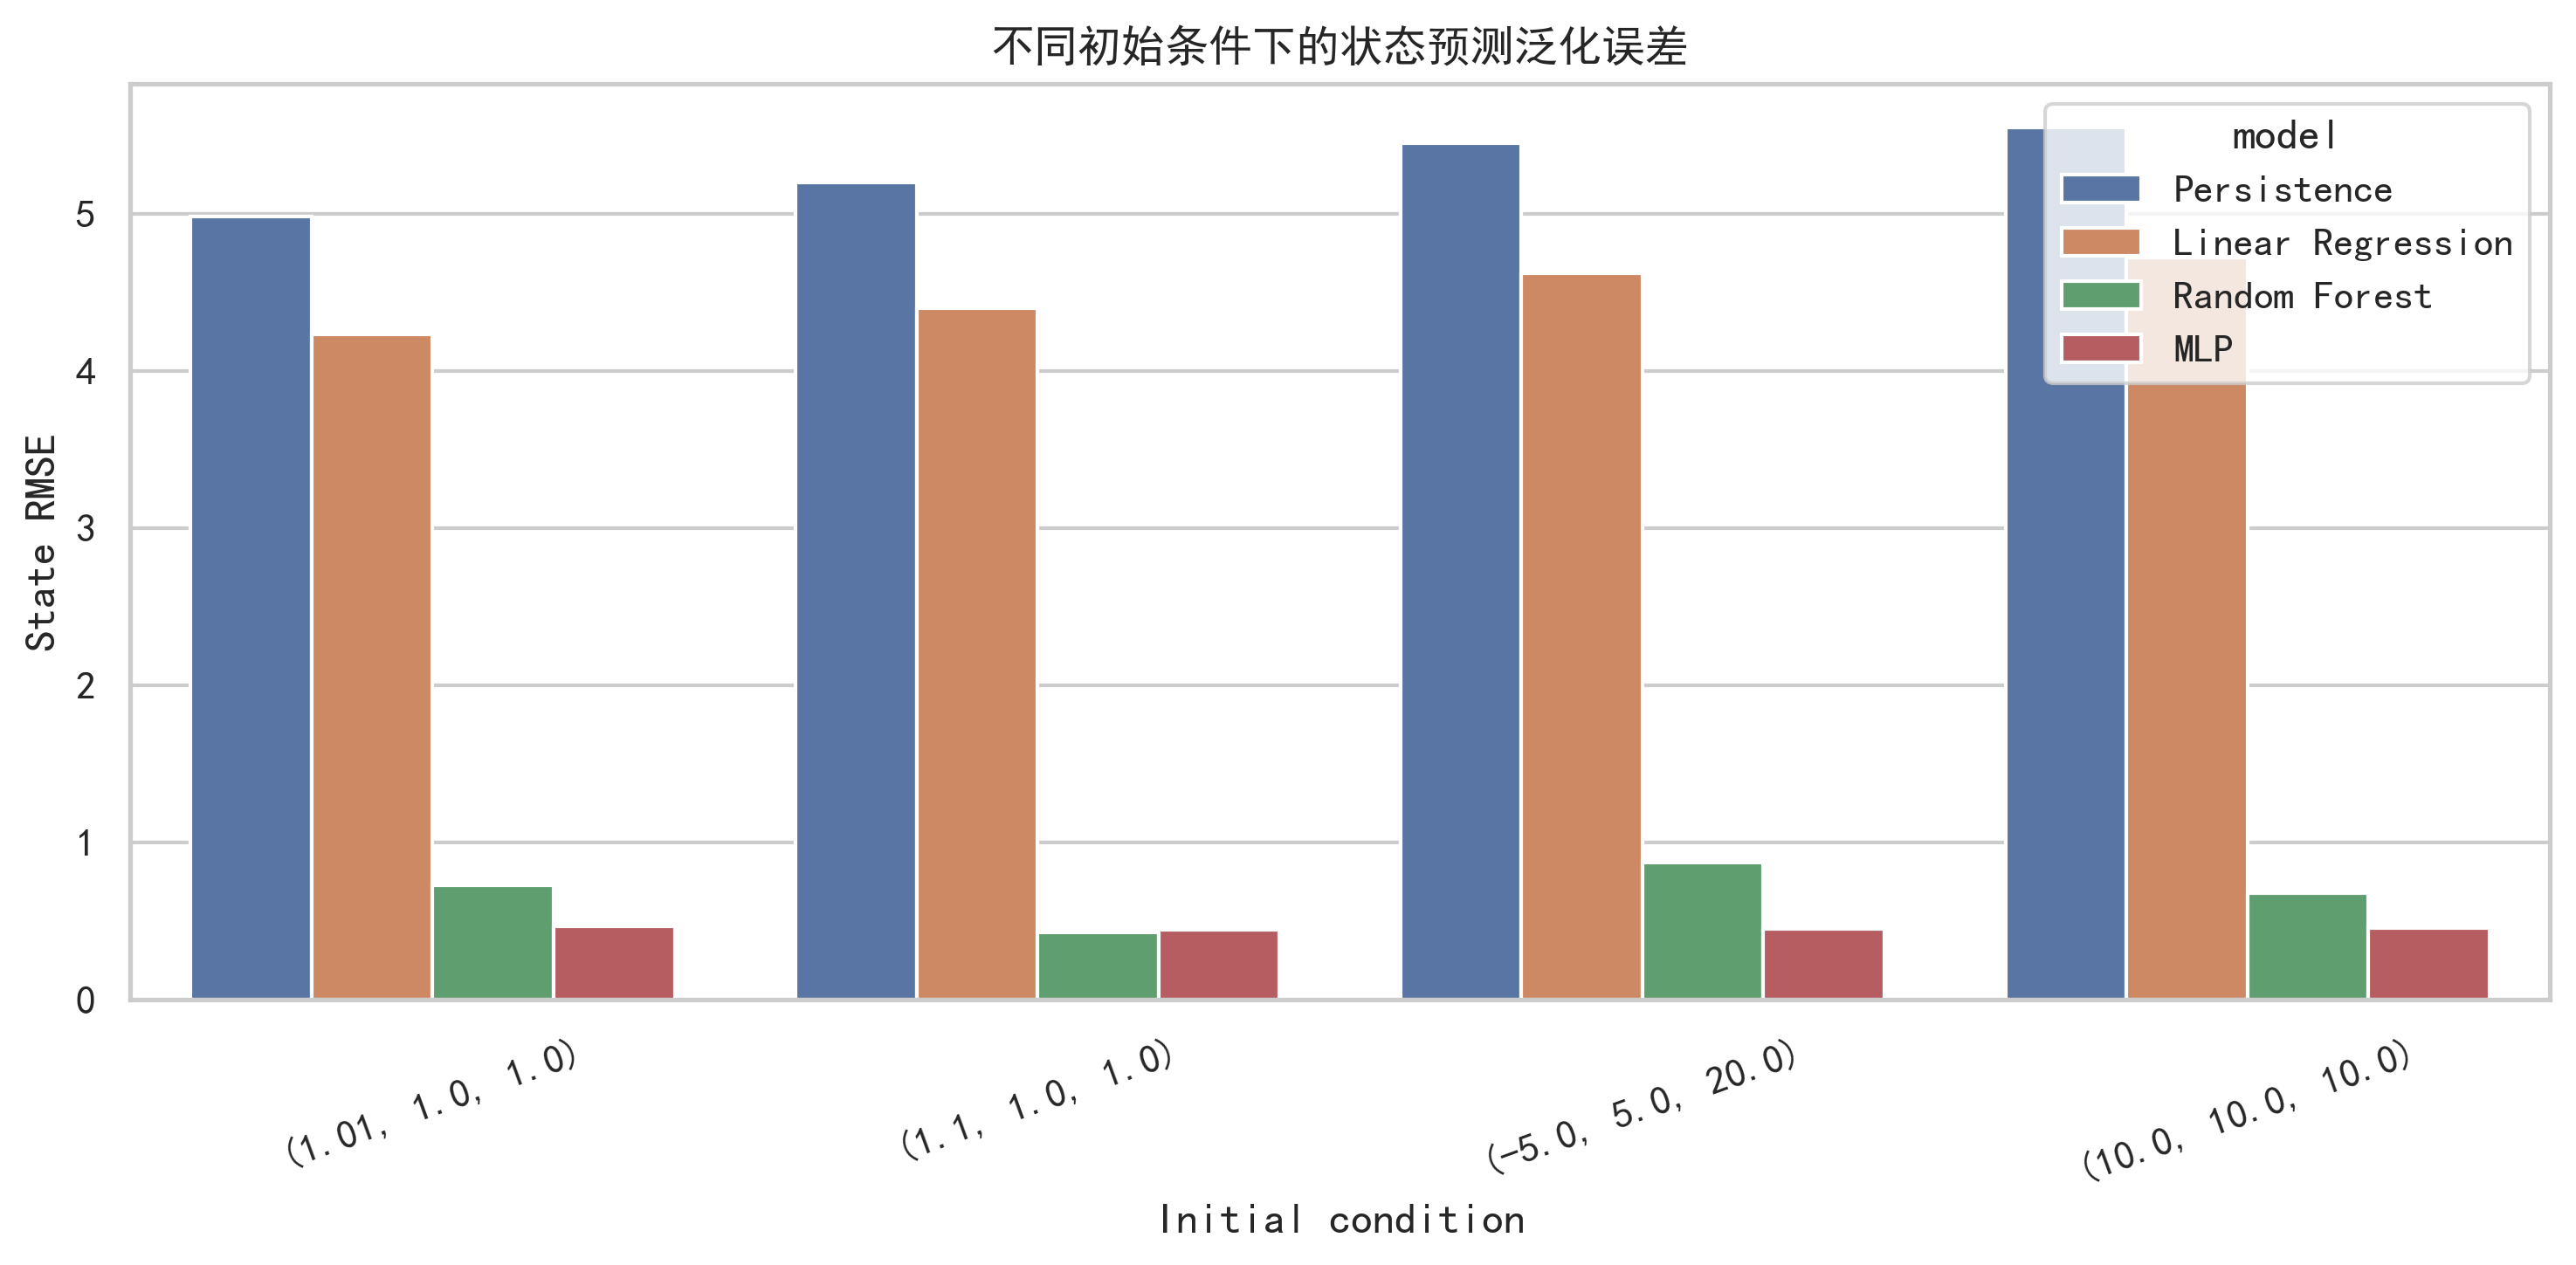
\includegraphics[width=0.88\textwidth]{figures/initial_condition_rmse.png}
\caption{不同初始条件下的状态预测泛化误差}
\label{fig:ic_rmse}
\end{figure}

\subsection{模型增强实验}

为了进一步分析什么样的模型结构更适合 Lorenz 系统的连续状态转移映射，本文加入输出标准化、Residual MLP、MLP 结构和激活函数消融，以及 Echo State Network 对照。表 \ref{tab:model_enhancement} 给出了代表性结果。

\begin{table}[H]
\centering
\caption{模型增强实验的代表性结果}
\label{tab:model_enhancement}
\begin{tabular}{rlcc}
\toprule
Horizon & 模型 & State RMSE & $R^2_{mean}$ \\
\midrule
10 & 原始 MLP & 0.4572 & 0.9991 \\
10 & Residual MLP ReLU 64-64-64 & 0.0772 & 0.99997 \\
10 & ESN residual & 0.4566 & 0.9991 \\
100 & 原始 MLP & 2.2369 & 0.9781 \\
100 & Residual MLP ReLU 64-64-64 & 1.4133 & 0.9913 \\
100 & ESN residual & 76.9877 & -26.0032 \\
500 & 原始 MLP & 13.6858 & 0.1591 \\
500 & Residual MLP ReLU 64-64 & 13.8243 & 0.1417 \\
500 & Random Forest baseline & 12.7868 & 0.2607 \\
\bottomrule
\end{tabular}
\end{table}

图 \ref{fig:model_enhancement} 展示了不同增强模型在 horizon=10、100、500 下的 state RMSE。结果表明，输出标准化和 residual learning 在短期和中期预测中明显改善 MLP 表现；其中更深的 ReLU residual MLP 在 horizon=10 和 horizon=100 上表现最好。但当 horizon 增大到 500 时，各类 MLP 都出现明显退化，Random Forest 反而保持相对较低误差。这说明模型结构改进可以扩大可预测时间窗，但不能消除混沌系统长期预测困难。

\begin{figure}[H]
\centering
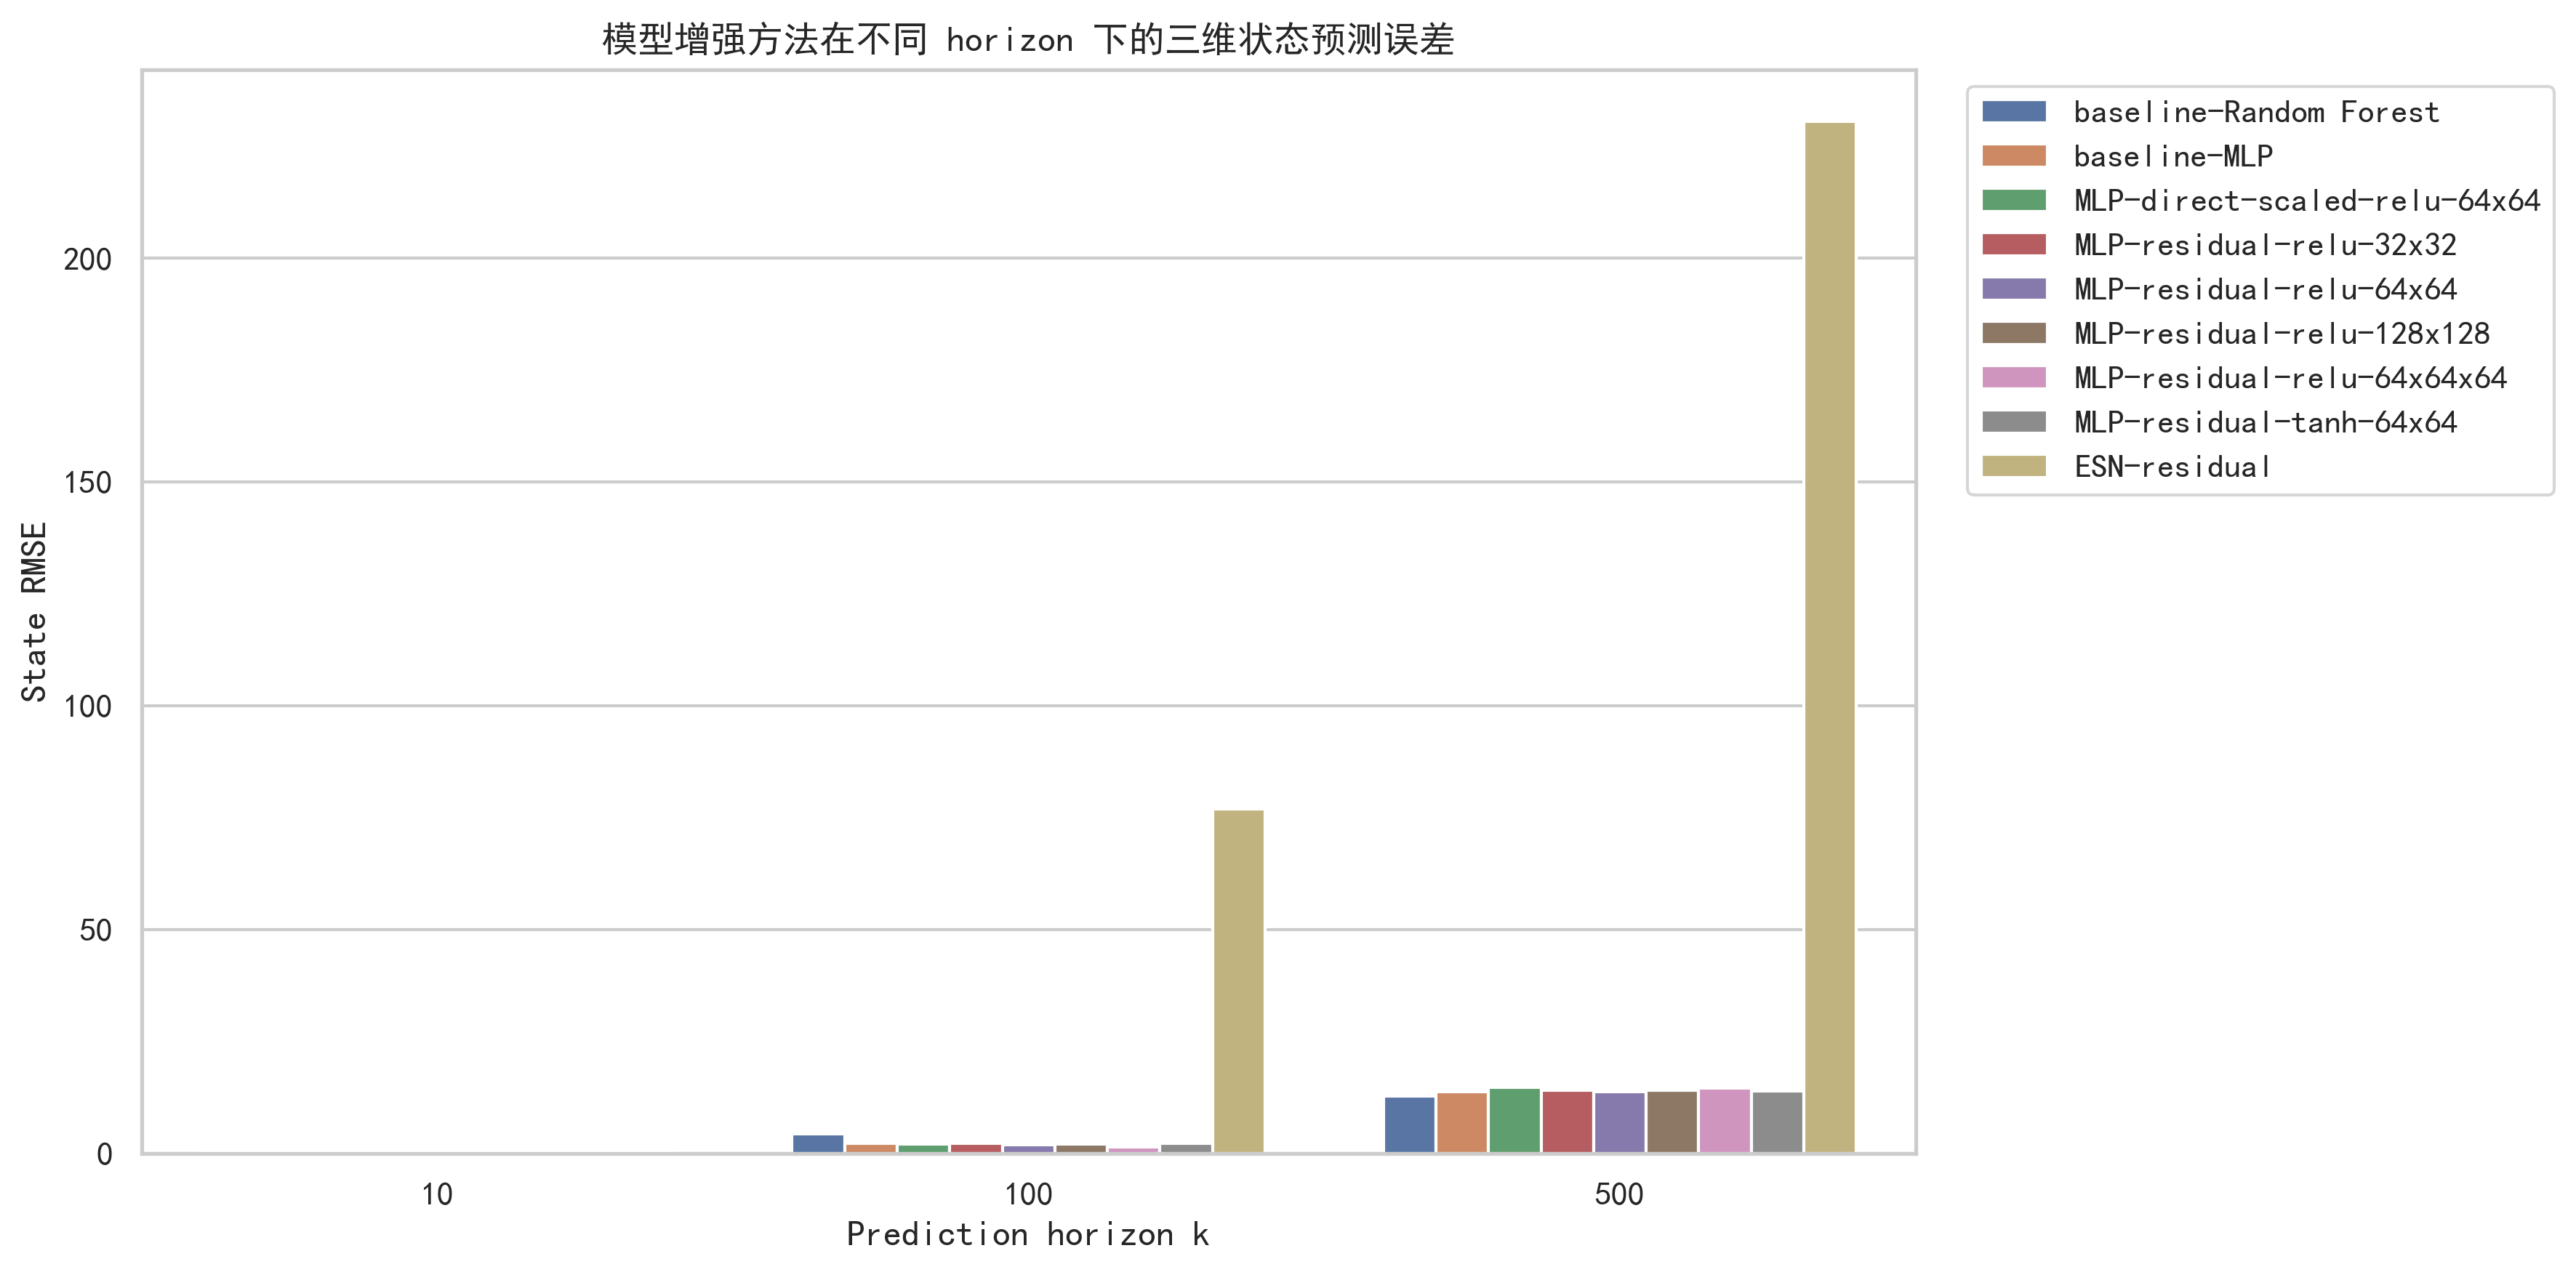
\includegraphics[width=0.95\textwidth]{figures/model_enhancement_horizon_rmse.png}
\caption{Residual MLP、输出标准化与 ESN 在不同 horizon 下的对比}
\label{fig:model_enhancement}
\end{figure}

图 \ref{fig:enhanced_rollout_error} 展示了增强模型在 500 步 recursive rollout 中的误差。Residual MLP tanh 64-64 的累计 state RMSE 约为 10.7975，优于原始 MLP rollout 的 18.0711；ESN residual 的累计 state RMSE 约为 14.7144，表现中等但提供了动力系统时间序列模型视角。

\begin{figure}[H]
\centering
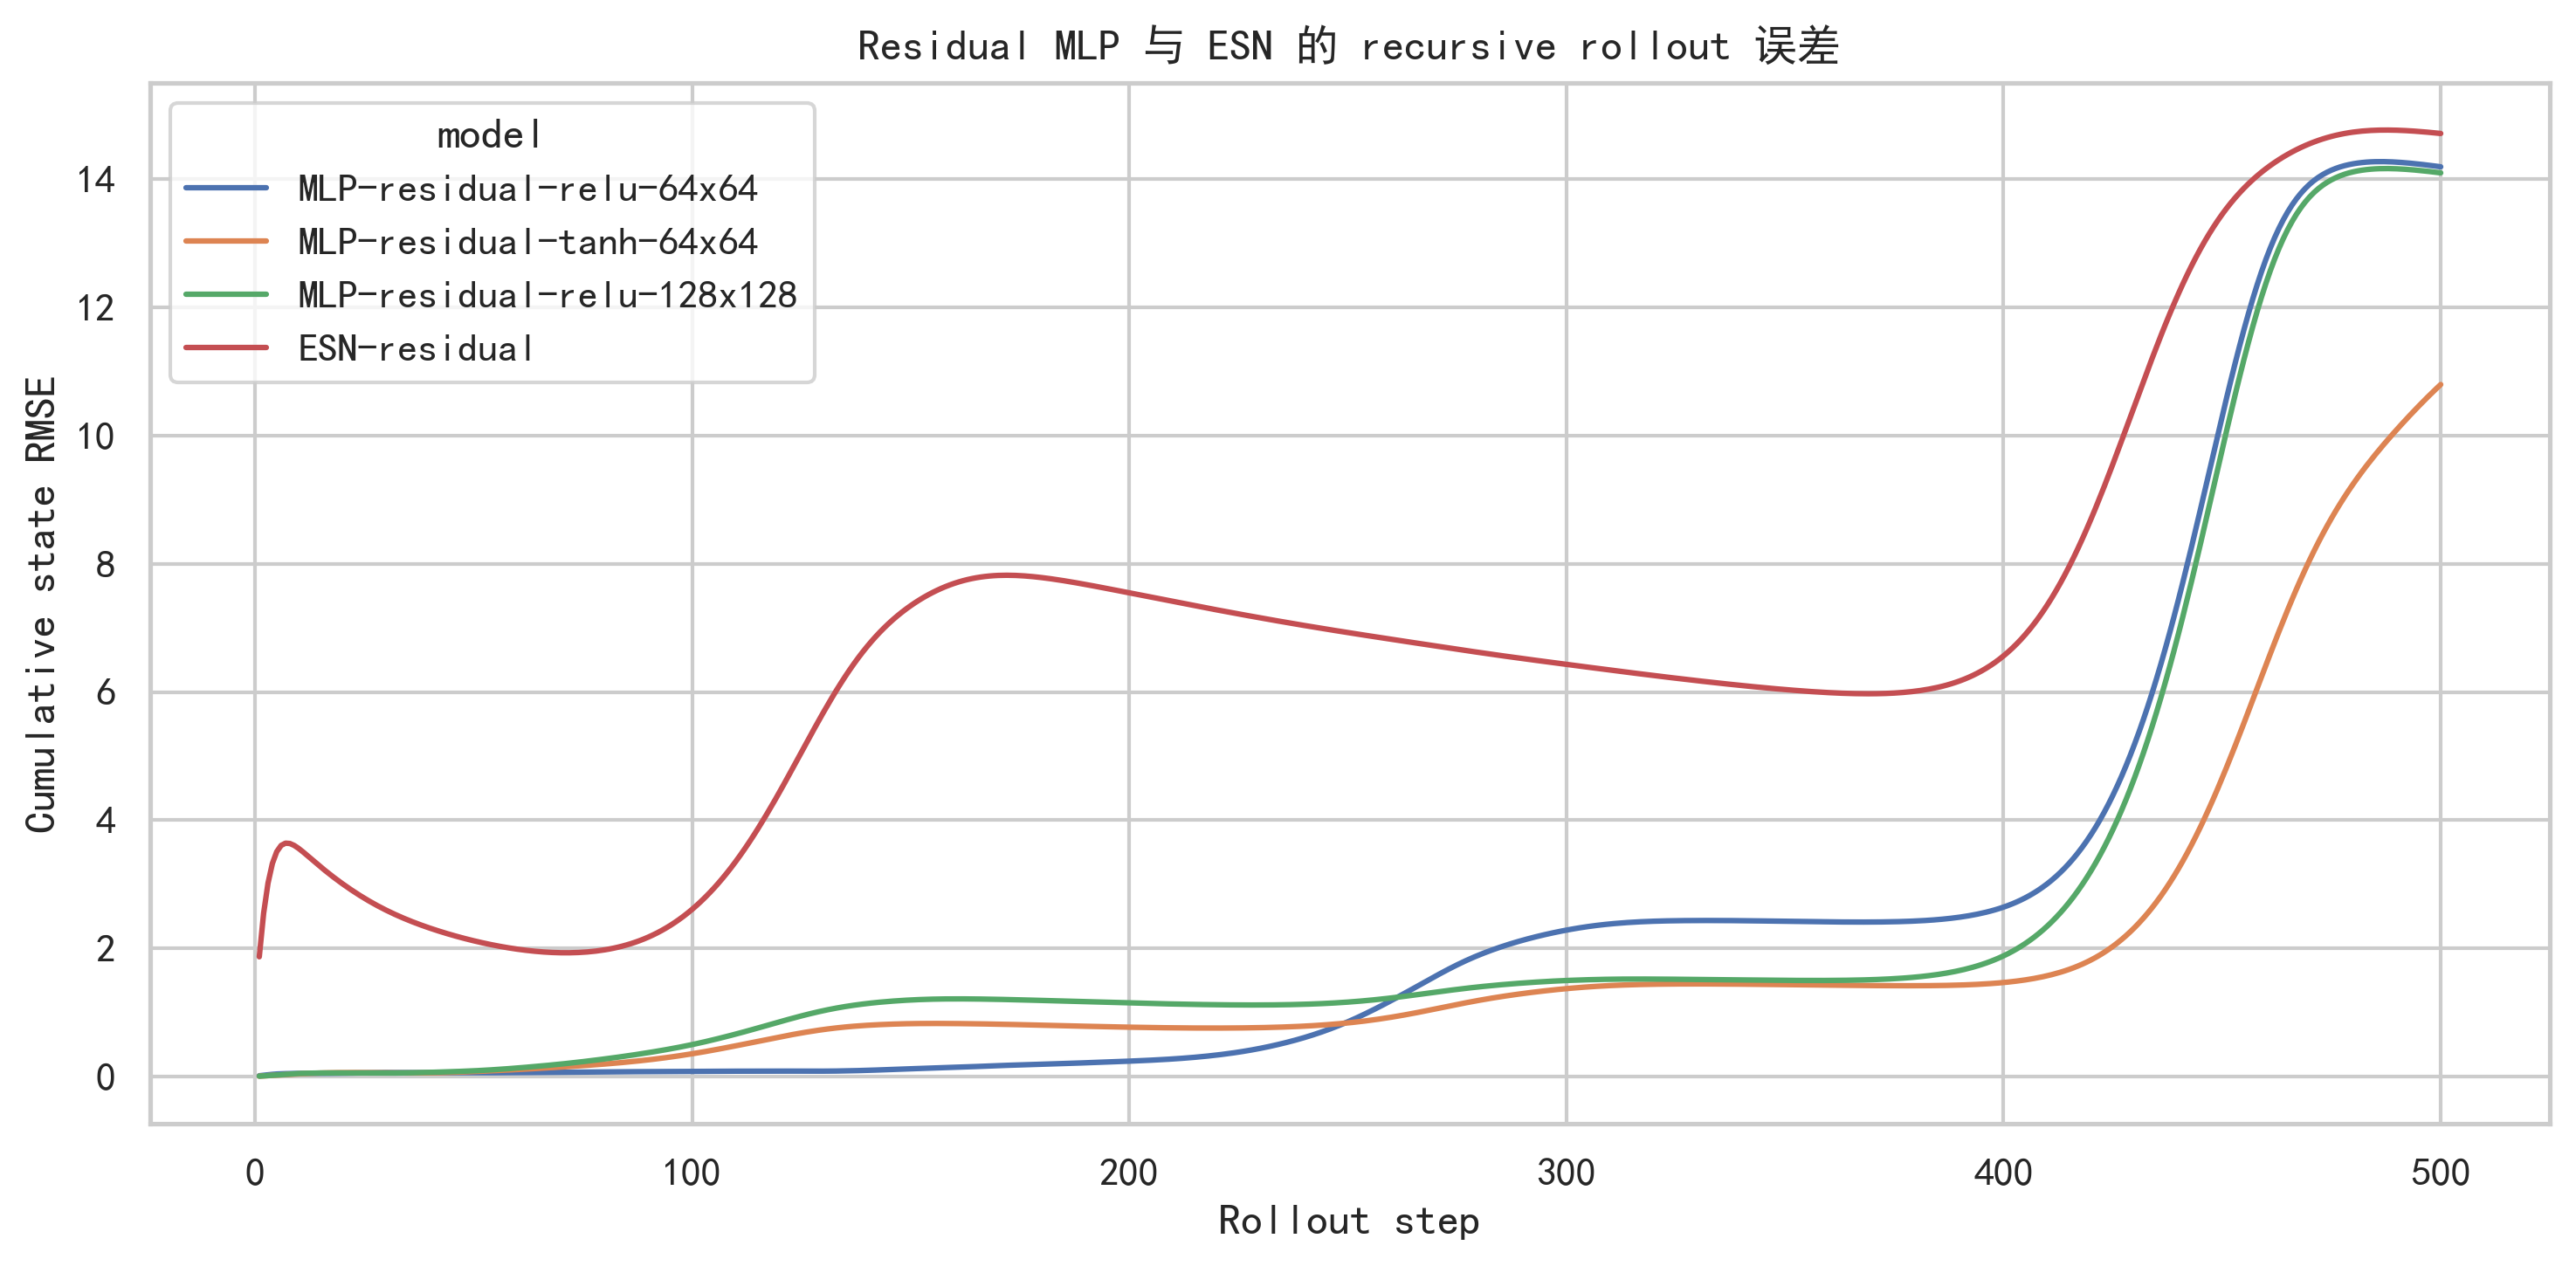
\includegraphics[width=0.88\textwidth]{figures/enhanced_rollout_error.png}
\caption{增强模型 recursive rollout 误差曲线}
\label{fig:enhanced_rollout_error}
\end{figure}

\begin{figure}[H]
\centering
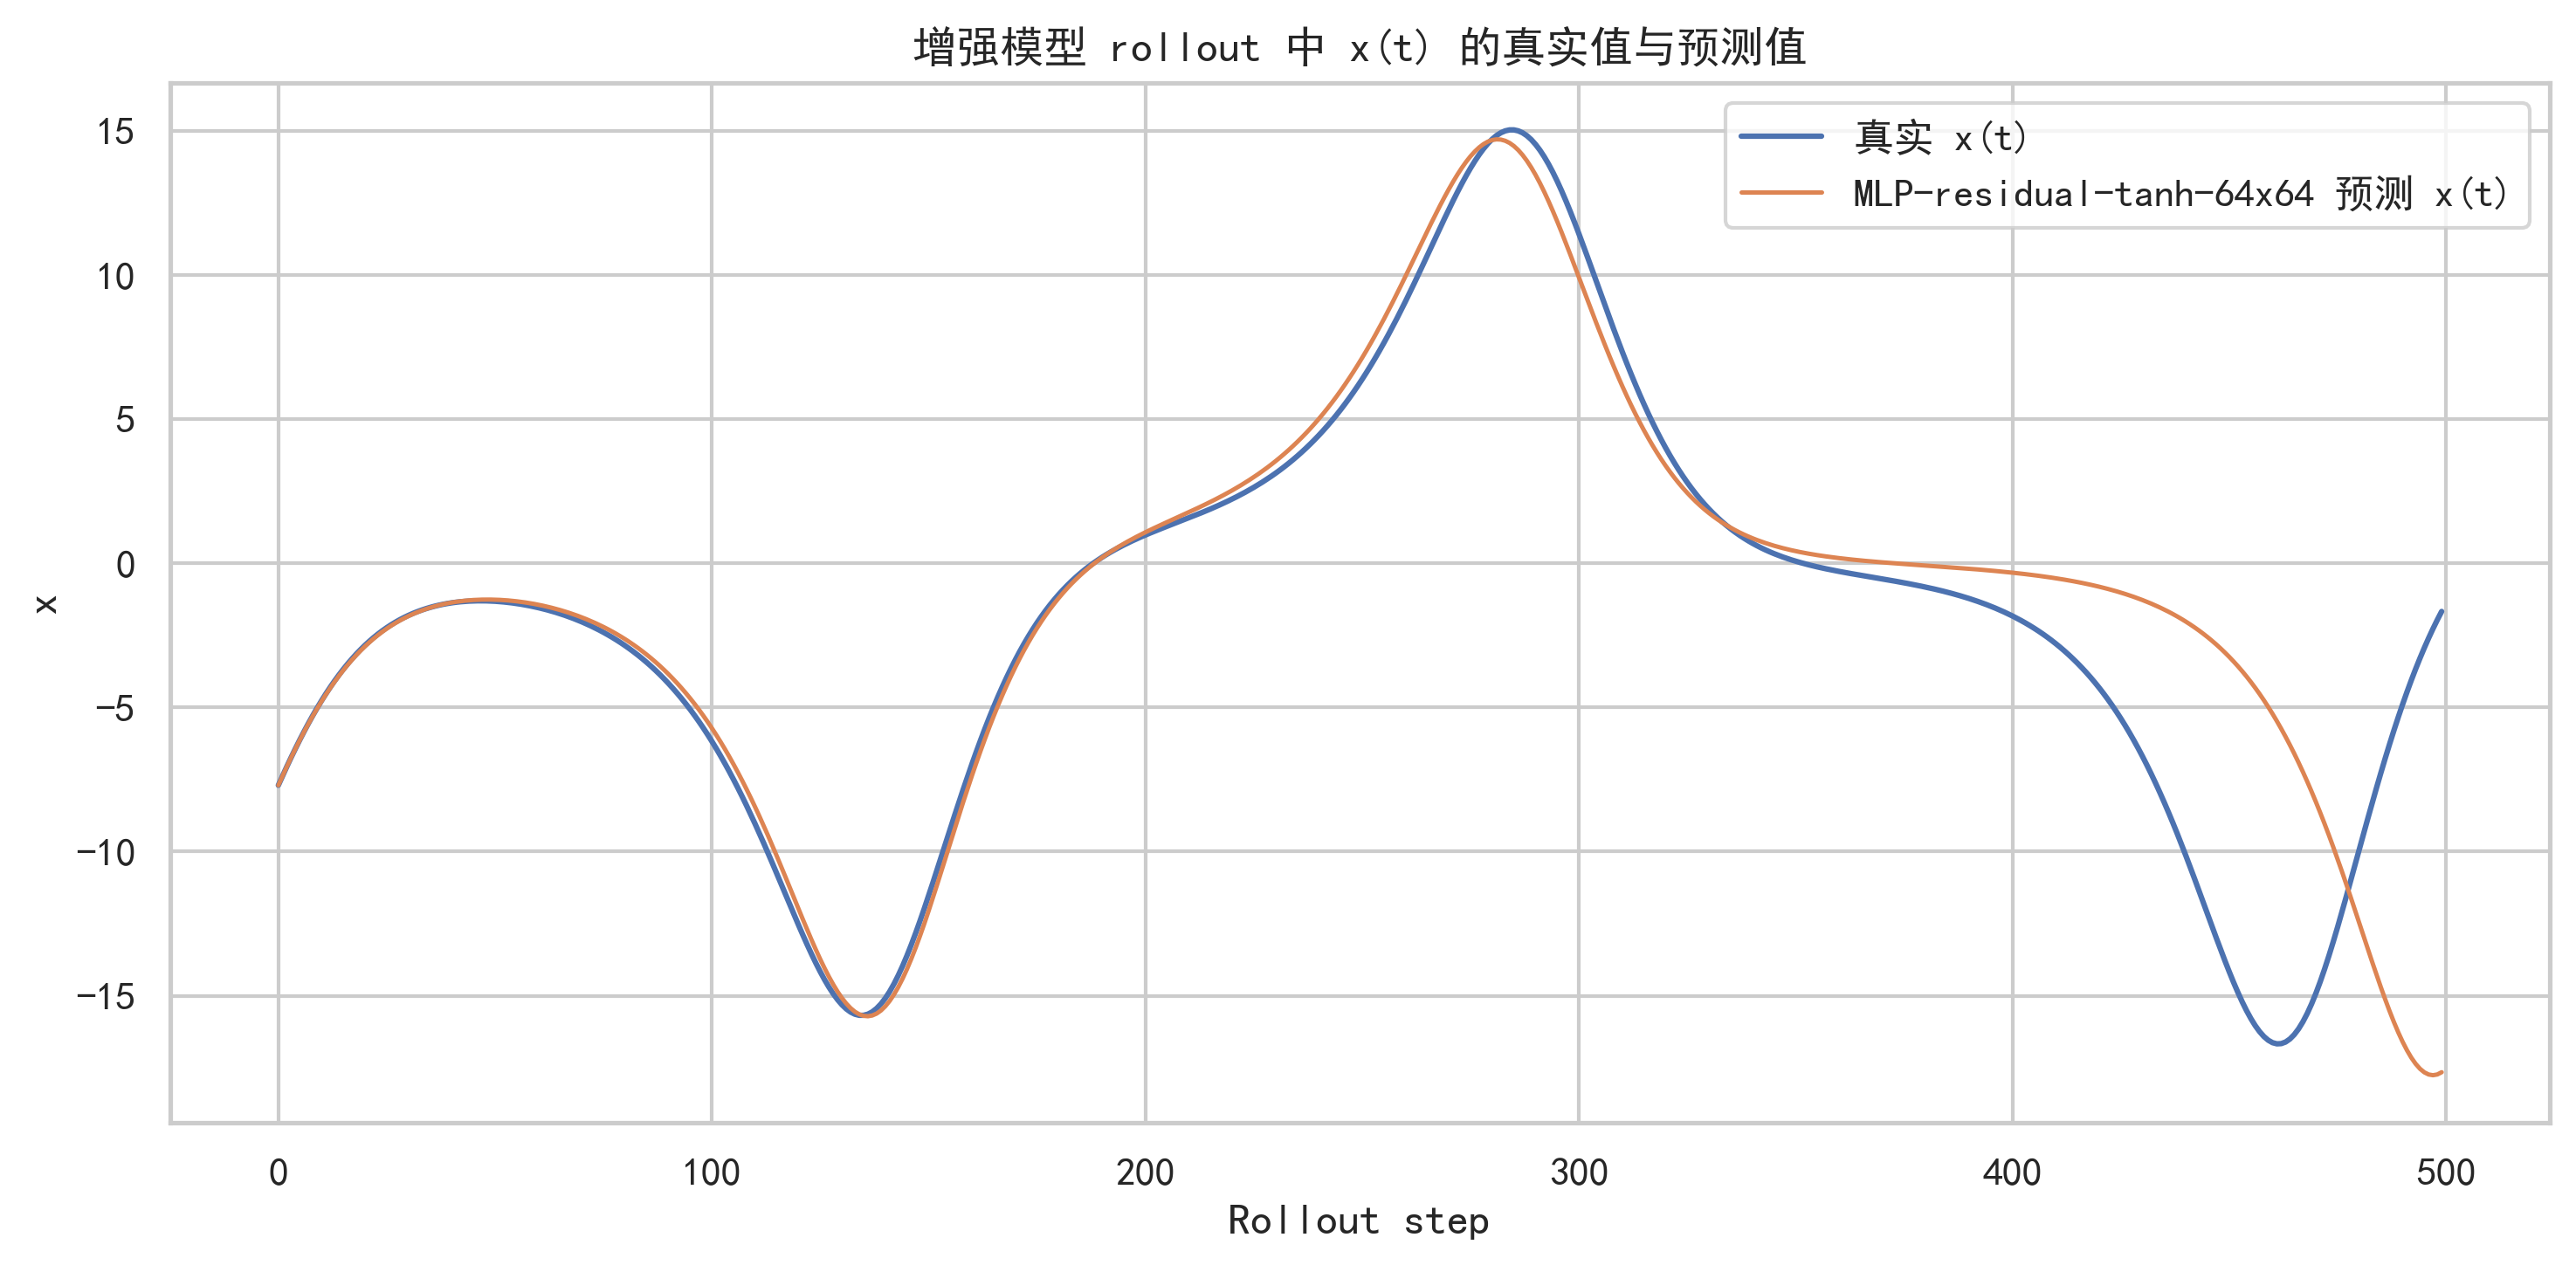
\includegraphics[width=0.88\textwidth]{figures/enhanced_rollout_x_comparison.png}
\caption{增强模型 rollout 中 $x(t)$ 的真实值与预测值对比}
\label{fig:enhanced_rollout_x}
\end{figure}

\section{讨论}

本文结果显示，Lorenz 系统的短期局部状态转移确实可以被机器学习模型有效逼近。尤其是在 horizon 较小时，Random Forest、MLP 和 Residual MLP 的 state RMSE 都较低，说明非线性模型能够从数据中学习局部状态映射。这一结果与 Lorenz 方程的连续性一致：在足够短的时间尺度内，系统状态不会发生任意跳变。

模型增强实验说明，模型结构本身也会影响预测边界。直接预测未来状态并不总是最自然的做法；对 Lorenz 这类连续动力系统，学习状态增量 $\Delta\mathbf{s}$ 更贴近数值积分思想。输出标准化也能改善 MLP 训练稳定性，避免某个状态分量因尺度较大而主导损失。消融结果显示，更深的 residual ReLU MLP 在 horizon=10 和 horizon=100 上更优，而 tanh residual MLP 在 rollout 中更稳定，这说明平滑激活函数可能更适合连续流映射。

ESN 的加入提供了动力系统时间序列模型视角，但本实验中的轻量 ESN 并没有全面超过 Residual MLP。尤其在较长 horizon 的 direct prediction 中，ESN residual 出现明显失效。这说明 reservoir computing 的效果依赖 reservoir 规模、谱半径、泄漏率和 readout 正则化等超参数，不能简单认为只要加入 ESN 就一定优于普通 MLP。

但是，本文更重要的发现仍然是预测能力存在边界。首先，prediction horizon 增大后，模型不再只是学习局部小步变化，而需要跨越更长时间的非线性演化，误差明显上升。其次，recursive rollout 中模型误差会被反复作为下一步输入，导致误差持续累积。最后，不同初始条件测试表明，模型在未重新训练时虽然有一定泛化能力，但泛化质量依赖于新轨迹是否仍处在训练数据覆盖较好的区域。

因此，不能把短期 $R^2\approx 1$ 解读为机器学习已经实现了混沌系统长期精确预测。更严谨的表述是：非线性机器学习模型能够近似 Lorenz 系统的短期局部状态转移映射；Residual learning、输出标准化和合适的激活函数能扩大部分可预测时间窗；但其长期预测能力仍受 prediction horizon、递归误差累积和初始条件敏感性共同限制。

\section{AI 协作反思}

本项目使用 LLM 辅助完成选题、建模路线设计、Notebook 结构规划、实验结果解释和报告撰写。LLM 的主要作用是帮助将课程要求组织为可复现的机器学习实验，并在发现原始任务研究性不足后，协助把项目扩展为 prediction horizon、recursive rollout 和 initial-condition generalization 三类更有研究意义的分析。

同时，LLM 生成的代码和文字必须由人工和实际运行结果验证。例如，Lorenz 方程、数据切分、StandardScaler 的 fit/transform 顺序、rollout 是否错误地使用真实未来状态、图表路径和 LaTeX 引用都需要人工检查。因此，本项目将 LLM 作为辅助工具，最终结论以可复现代码和实验输出为准。

\section{结论}

本文将 Lorenz 混沌系统机器学习预测项目从单一 $x(t+10\Delta t)$ 短期预测扩展为完整三维状态转移预测，并新增 prediction horizon sensitivity、recursive multi-step rollout、initial-condition generalization 和模型结构增强实验。实验表明，非线性机器学习模型可以在短 prediction horizon 下较好近似 Lorenz 系统的局部状态转移映射；Residual MLP 和输出标准化能显著改善中短期状态预测；tanh residual MLP 在本实验的 rollout 设置中更稳定；ESN 提供了动力系统时间序列模型对照，但需要进一步调参才能充分发挥优势。

然而，随着 horizon 增大，直接预测误差仍显著上升；在 recursive rollout 中，一步预测误差会不断累积；在不同初始条件轨迹上，模型泛化能力也会受到训练数据覆盖范围限制。因此，本文结论不是“机器学习成功解决混沌系统预测”，而是：The results show that nonlinear machine learning models can approximate the local state-transition map of the Lorenz system under short prediction horizons. Residual learning and output scaling can improve short- and medium-horizon prediction, but prediction errors still grow as the horizon increases and under recursive multi-step forecasting, reflecting the intrinsic difficulty of long-term prediction in chaotic systems.

未来工作可以进一步引入噪声鲁棒性测试、跨参数泛化实验、horizon-conditioned MLP，以及对 Echo State Network / Reservoir Computing 的 reservoir 规模、谱半径、泄漏率和正则化系数进行系统调参。

\begin{thebibliography}{99}

\bibitem{lorenz1963}
Lorenz, E. N. (1963).
Deterministic nonperiodic flow.
\textit{Journal of the Atmospheric Sciences}, 20(2), 130--141.

\bibitem{pedregosa2011}
Pedregosa, F., Varoquaux, G., Gramfort, A., Michel, V., Thirion, B., Grisel, O., Blondel, M., Prettenhofer, M., Weiss, R., Dubourg, V., Vanderplas, J., Passos, A., Cournapeau, D., Brucher, M., Perrot, M., \& Duchesnay, E. (2011).
Scikit-learn: Machine learning in Python.
\textit{Journal of Machine Learning Research}, 12, 2825--2830.

\bibitem{virtanen2020}
Virtanen, P., Gommers, R., Oliphant, M., Haberland, M., Reddy, T., Cournapeau, D., Peterson, P., Weckesser, W., Bright, J., van der Walt, S., Brett, M., Wilson, J., Millman, K., Mayorov, N., Nelson, A., Jones, E., Kern, R., Larson, E., Carey, C., Polat, I., Feng, Y., Moore, E., VanderPlas, J., Laxalde, D., Perktold, J., Cimrman, R., Henriksen, I., Quintero, E., Harris, C., Archibald, A., Ribeiro, A., Pedregosa, F., \& van Mulbregt, P. (2020).
SciPy 1.0: Fundamental algorithms for scientific computing in Python.
\textit{Nature Methods}, 17, 261--272.

\bibitem{strogatz2015}
Strogatz, S. H. (2015).
\textit{Nonlinear Dynamics and Chaos: With Applications to Physics, Biology, Chemistry, and Engineering}.
Westview Press.

\bibitem{lukosevicius2009}
Luko\v{s}evi\v{c}ius, M., \& Jaeger, H. (2009).
Reservoir computing approaches to recurrent neural network training.
\textit{Computer Science Review}, 3(3), 127--149.

\end{thebibliography}

\appendix

\section{大模型交互与提示词工程实录}

本项目使用 LLM 作为辅助工具参与以下环节：

\begin{enumerate}
    \item 根据课程要求筛选 AI4SCI 与数学建模方向选题；
    \item 将 Lorenz 混沌系统转化为监督学习回归任务；
    \item 设计 Persistence、Linear Regression、Random Forest、MLP 等模型角色；
    \item 发现原始单变量短期预测任务研究性不足，并提出 prediction horizon、recursive rollout 和 initial-condition generalization 增强实验；
    \item 进一步提出 Residual MLP、输出标准化、MLP 消融和 Echo State Network 作为模型层面的增强；
    \item 辅助生成 Notebook 代码结构、图表保存逻辑和 LaTeX 报告框架。
\end{enumerate}

代表性提示词包括：

\begin{enumerate}
    \item “选择 Lorenz 混沌系统作为项目题目，并设计机器学习建模路线。”
    \item “请加入标准化、回归模型和 RMSE/MAE/$R^2$ 评价指标。”
    \item “这个论文根本没有研究什么，思考如何改进。”
    \item “把项目增强为 prediction horizon、三维状态预测、recursive rollout 和跨初始条件泛化分析。”
    \item “比较 Direct MLP、Residual MLP、输出标准化、激活函数和 Echo State Network。”
\end{enumerate}

\end{document}
